\documentclass[12pt,a4paper]{article}
\usepackage[utf8]{inputenc}
\usepackage[russian]{babel}
\usepackage{amsmath}
\usepackage{amsfonts}
\usepackage{amssymb}
\usepackage{caption}
\usepackage{subcaption}
\usepackage{graphicx}
\usepackage{textcomp}
\author{Хасан Хафизов}
\title{Децентрализованное управление строем}

\begin{document}
	\maketitle

\section{Постановка задачи}


\section{Механическая модель агента}
Моделью агента является материальная точка с массой $m$. Закон движения:
$$\begin{cases} 
m \ddot{x} = F_x \\
m \ddot{y} = F_y \end{cases}
$$

$\vec{F}$ — сила, действующая на агента, может включать в себя:
$$ \vec{F} = \vec{u} + \vec{W} + \vec{F_{\text{тр}}}$$
Где $\vec{u}$ — управляющее воздействие, $\vec{W}$ — случайные помехи, $\vec{F_{\text{тр}}}$ — сила трения.
\par
В предлагаемом мной алгоритме управления агентов можно разделить на два класса:
\begin{itemize}
	\item интеллектуальный (мастер)
	\item управляемый (миньон)
\end{itemize}
Закон управления для этих двух типов агентов задаётся по-разному.
\subsection{Мастер}
Мастером является агент, для которого желаемый закон движения $S_d$ задаётся оператором извне: это может быть записанная в память агента траектория, целевая позиция или скорость. \par
Фактически, этот агент ничего не знает о существовании других агентов в строю (миньонов). Его задача — выполнение поставленного закона движения, поэтому закон управления зависит только от закона движения:
$$ \vec{u} = \vec{u}(S_d)$$
Рассмотрим конкретный закон управления $\vec{u}_{tr}$: движение по некоторой траектории $\vec{tr}(t)$:
$$ \vec{u}_{tr} = \vec{u}_{along} + \vec{u}_{across} $$
Закон управления состоит из двух частей. Первая $\vec{u}_{along}$ отвечает за усилие вдоль траектории, вторая $\vec{u}_{across}$ — поперёк. Направлением для $\vec{u}_{along}$ служит направление вектора между текущим положением агента и следующей точкой траектории.
\begin{center}{\textit{ (Тут будет более подробно о том, как вычисляется следующая точка траектории, о алгоритмах управления на PD регуляторах, которые используются как в $\vec{u}_{along}$, так и в $\vec{u}_{across}$)}}
\end{center}
Пример движения мастера по траектории, задаваемой параметрическим уравнением, где $s$ — параметр: $s \in [0, 5000]$.
$$x(s) = 300 \cdot \cos(\frac{s}{300}); \ y(s) = s$$

\begin{figure}[!htbp]
	\centering
	\begin{subfigure}{.5\textwidth}
		\centering
		
\includegraphics[width=1\linewidth]{master-trajectory-0}
		\caption{Исходная траектория и след от движения}
		\label{fig:sub1}
	\end{subfigure}%
	\begin{subfigure}{.5\textwidth}
		\centering
		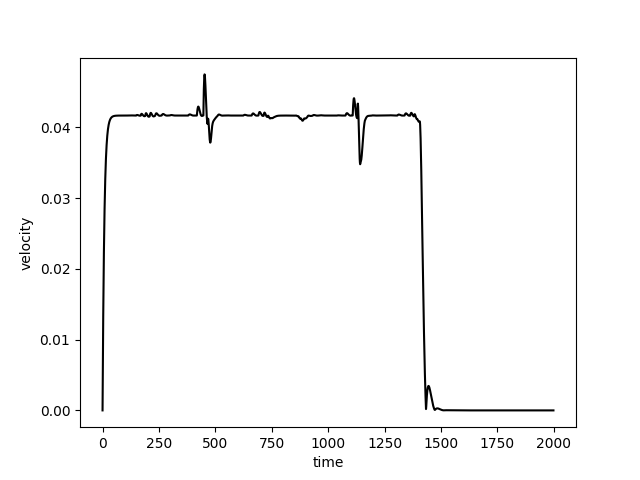
\includegraphics[width=1\linewidth]{master-trajectory-0-velocity}
		\caption{Скорость движения мастера}
		\label{fig:sub2}
	\end{subfigure}
	\caption{Движение мастера по заданной траектории с заданной скоростью $\upsilon_{desired} = 20 \frac{\text{м}}{\text{с}}$. Расстояния на рисунках задаются в метрах, время в секундах, скорость в $\frac{\text{м}}{\text{с}}$}.
	\label{fig:test}
\end{figure}
\subsubsection{Оценка движения мастера по траектории}
Агент преодолел заданную траекторию за $t = 331 \text{с}$. \\
Проеденное расстояние:
$$ S = \int_{0}^{5000} \sqrt{x'^2(s) + y'^2(s)} \ ds \approx 6051 \text{м} $$ \\
Средняя скорость $\upsilon_{av} = 18.3  \frac{\text{м}}{\text{с}}$. \\
Стационарным режимом движения можно назвать режим, при котором скорость агента колеблется в пределах между $18.8\frac{\text{м}}{\text{с}}$ и $21.5\frac{\text{м}}{\text{с}}$. Более подробно скорость мастера в стационарном режиме можно увидеть на рис. \ref{fig:errors-master}a \\

\begin{figure}[!htbp]
	\centering
	\begin{subfigure}{.5\textwidth}
		\centering
		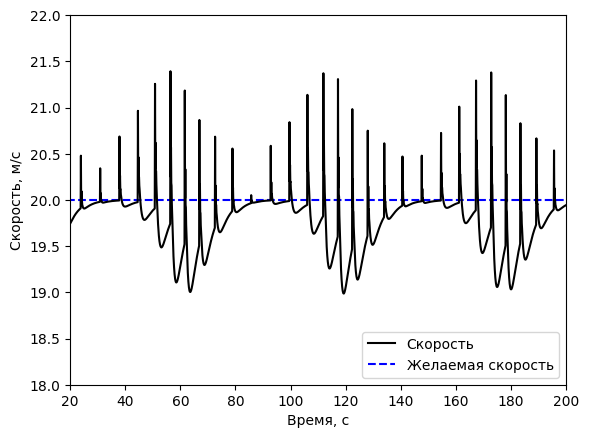
\includegraphics[width=1\linewidth]{master-trajectory-1-velocity.png}
		\caption{Скорость мастера в стационарном режиме}
		\label{fig:error-master-1}
	\end{subfigure}%
	\begin{subfigure}{.5\textwidth}
		\centering
		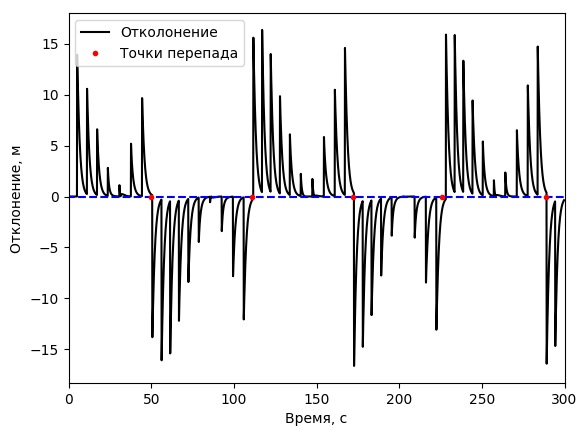
\includegraphics[width=1\linewidth]{master-trajectory-error.png}
		\caption{Отклонения мастера от траектории}
		\label{fig:error-master-2}
	\end{subfigure}
	\caption{Иллюстрация отклонений от желаемого закона движения}.
	\label{fig:errors-master}
\end{figure}
Отклонения агента от заданной траектории представлены на рис. \ref{fig:errors-master}b. Выше нуля — отклонения от траектории вправо, ниже нуля — влево. Максимальное отклонение составляет примерно 15 м. \par
Резкие перепады на графике, обозначенные как точки перепада объясняются тем, что в этих точках у траектории изменяется знак первой производной, а агент, всегда остающийся на внутренней части траектории резко оказывается на внешней. Проверим это утверждение. Заданное выше параметрическое уравнение фактически является уравнением $$x = 300 \cdot \cos(\frac{y}{300})$$
Равенство нулю первой производной:
$$\sin(\frac{y}{300}) = 0 \Rightarrow y = 300 \pi n$$
Найдём первые 5 точек траектории, в которой происходит смена знака второй производной: $$M = \Big\{(-300; \ 942), \ (300; \ 1885), \ (-300; \ 2827), \ (300; \ 3770), \ (-300; \ 4712)\Big\}$$
Найдём моменты времени, в которые эти точки будут достигнуты агентом:
$$\hat{L_t} = \Big\{ 61c, \ 118c, \ 177c, \ 234c, \ 292c \Big\}$$
Реальные же моменты времени, в которые просходит резкое изменение величины отклонения от траектории:
$${L_t} = \Big\{ 50c, \ 110c, \ 172c, \ 226c, \ 289c \Big\}$$
То есть, изменение стороны относительно линии траектории по которой движется агент изменяется незадолго до того, как будет изменён знак первой производной траектории. Эта закономерность так же наблюдается на рис. \ref{fig:master-trajectory-changes-2}. \par
\begin{figure}[!htbp]
	\centering
	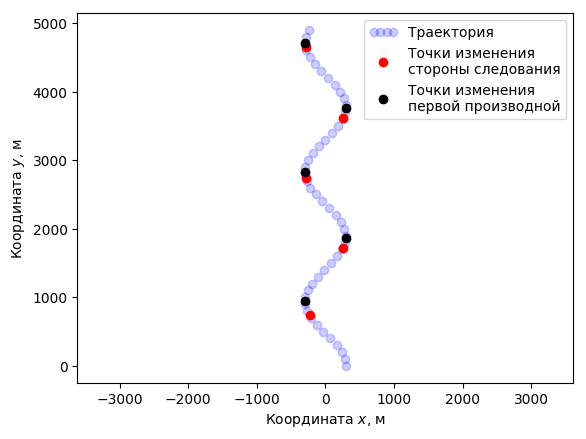
\includegraphics[width=0.5\linewidth]{master-trajectory-changes-2}
	\caption{Траектория с наложенными на неё точками изменения стороны следования и точками изменения знака первой производной.}
	\label{fig:master-trajectory-changes-2}
\end{figure}

\begin{center}{\textit{ (Тут будет исседование устойчивости алгоритма к случайным возмущениям)}}
\end{center}

Выводы: движение мастера по траектории является точным и предсказуемым. Данный алгоритм управления по траектории с задаваемой скоростью является пригодным для применения.



\subsection{Миньон}
Миньон является ведомым агентом, он не имеет информации о траектории движения. 
\par
Расчёт местоположения виртуального лидера просходит следующим образом:
\begin{enumerate}
	\item Получение текущих координат от агента, являющегося 
\end{enumerate}

\section{Строй}

Строй представляет из себя множество агентов соединённых связями, подобно графу. Для каждого агента, не являющегося мастером должно быть определено не менее одного агента-лидера. Лидером для агента может быть как мастер, так и любой миньон. Каждый агент — вершина графа, каждая связь миньон-лидер — ребро графа. Пример строя из 5-ти агентов изображён на рис.\ref{fig:wedge-platoon}. \par
\begin{figure}[!htbp]
	\centering
	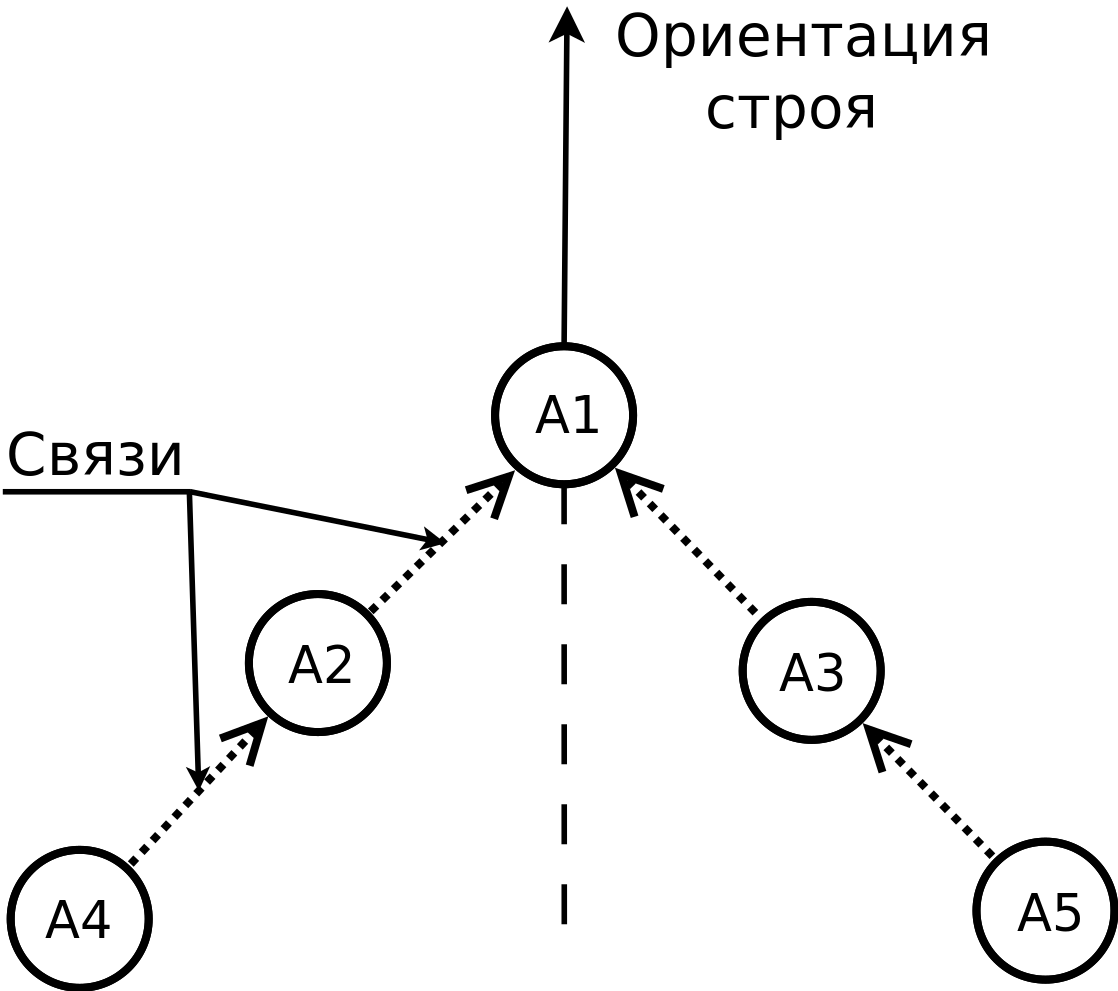
\includegraphics[width=0.5\linewidth]{platoon/wedge-platoon}
	\caption{Пример клиновидного строя из 5-ти агентов}
	\label{fig:wedge-platoon}
\end{figure}
Каждая связь $J_{ij}$ — это вектор в полярных координатах, у которого радиус — это расстояние от миньона $i$ до миньона лидера $j$, а угол — это угол между изначальной ориентацией строя и вектором, соединяющим миньона с его лидером. К примеру, если расстояния между каждой парой агентов равно 1м, то связи:
\begin{itemize}
	\item $J_{1j}$ — не определены ни для каких $j$: $A_1$ является мастером
	\item $J_{21} = (r=1\text{м}; \varphi=225\text{\textdegree{}})$ — для миньона $A_2$ агентом лидером является мастер $A_1$. Агенты находятся на расстоянии 1м, угол между соединяющим их вектором и вектором изначальной ориентации составляет $225 \text{\textdegree}$
	\item $J_{31}, J_{42}, J_{53}$ — определяются аналогично
\end{itemize}
При повороте строя поворачивается и вектор ориентации строя, за счёт чего далее пересчитывается позиция, в которой должен находиться агент после поворота. Эта позиция будет именоваться виртуальным лидером. Виртуальный лидер — точка пространства, в которую стремиться попасть миньон для того, чтобы поддерживать фигуру строя. \par
Например, на рис. \ref{fig:wedge-platoon-rotation} изображён поворот строя на угол $b$. Для того, чтобы пересчитать позицию, в которой должен находиться миньон после поворота (виртуальный лидер) необходимо повернуть вектор изначальной ориентации $O_{0}$ на угол $b + \varphi$, где $\varphi$ — угол из любого вектора связи $J_{ij}$ миньона $i$, далее от положения выбранного миньона-лидера необходимо отложить расстояние равное $r$ из вектора связи в направлении повёрнутого вектора изначальной ориентации $O_0$. 
\par
\begin{figure}[!htbp]
	\centering
	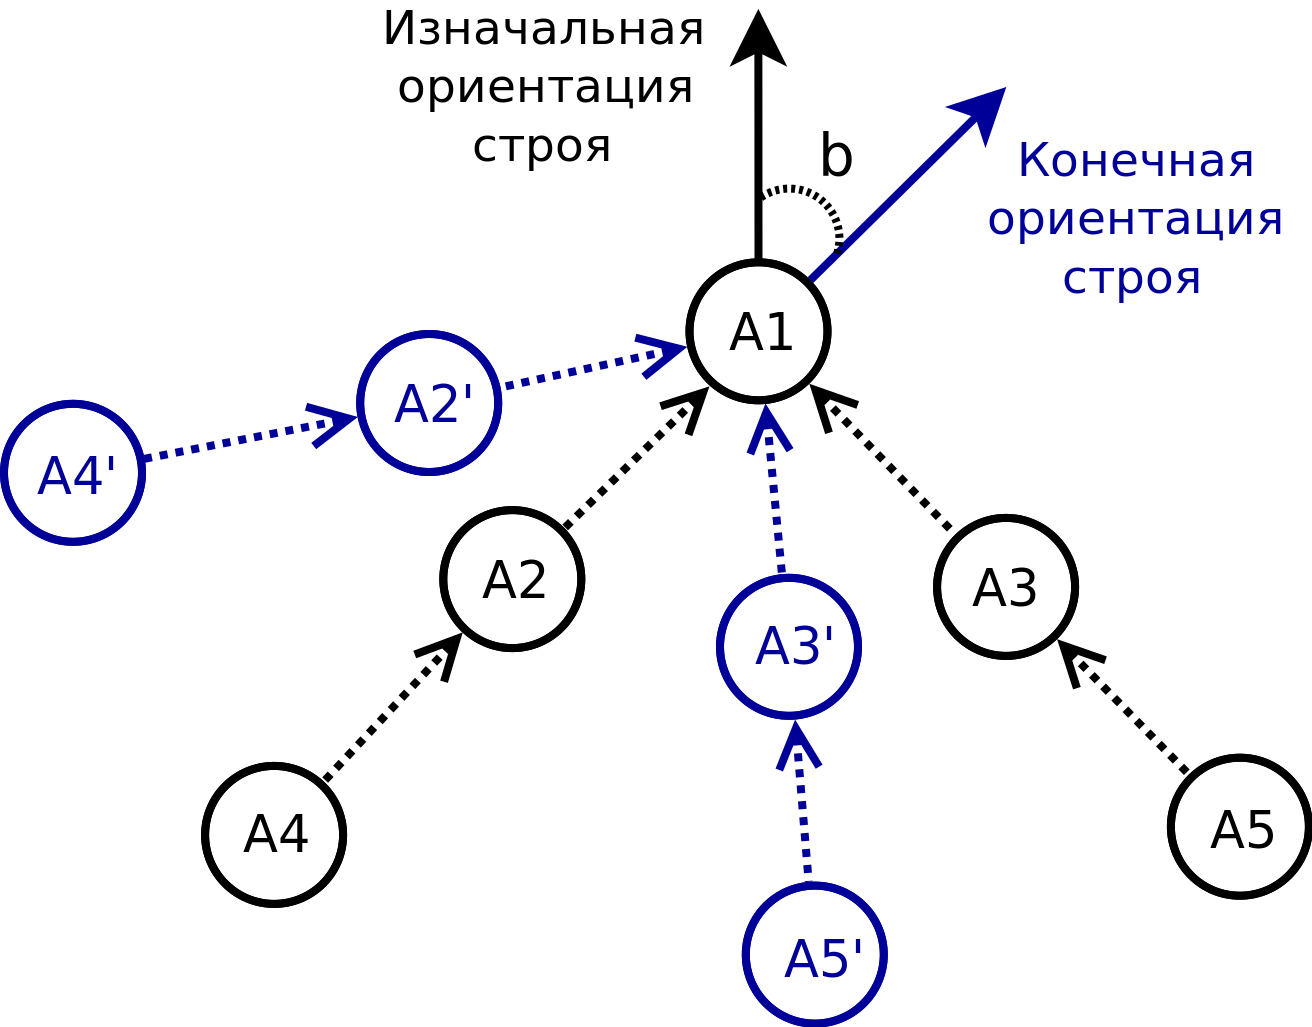
\includegraphics[width=0.5\linewidth]{platoon/wedge-platoon-rotation}
	\caption{Поворот строя на угол $b$}
	\label{fig:wedge-platoon-rotation}
\end{figure}
Рассмотрим пример того, как будет расчитан виртуальный лидер $A_5'$ для агента $A_5$ (см. рис. \ref{fig:wedge-platoon-rotation}), для которого определён вектор связи $J_{53} = (r_{53}; \ \varphi_{53})$ (вектор связи с $A_3$). Для начала повернём вектор изначальной ориентации $O_{0}$:
$$\vec{O_{1}} =  \left(\begin{array}{cc} \cos{(b + \varphi_{53})} & \sin{(b + \varphi_{53})}\\ \sin{(b + \varphi_{53})} & \cos{(b + \varphi_{53})} \end{array}\right) \vec{O_{0}} $$
Теперь вдоль полученного вектора $\vec{O_1}$ необходимо отложить от позиции агента $A_3$ расстояние равное $r_{53}$:
$$ \vec{A'_{5}} = \vec{A_3} + \frac{\vec{O_1}}{|\vec{O_1}|} r_{53}$$
\par
В приведённых выше расчётах неявно предполагалось, что агент $A_3$ на момент пересчёта виртуального лидера для $A_5$ уже находится в точке $A'_3$. До тех пор, пока не будет выполнено это условие получаемое $A'_5$ не будет совпадать с тем, что приведено на рисунке. Однако, это ожидаемая ситуация, т.к. $A_5$ не знает ни о каких агентах кроме $A_3$, то он и полагается только на данные, получаемые от $A_3$, а если $A_3$ ещё не достиг точки виртуального лидера, то и в координтах виртуального лидера $A'_5$ будут содержаться ошибки. \par
Описанную выше проблему несложно решить, если строить виртуальных лидеров на основе позиции не агента-лидера, а на основе точки виртуального лидера агента-лидера. Однако, после поворота у миньонов находящихся дальше от центра поворота (центр поворота — мастер) расстояние до их виртуальных лидеров окажется больше, чем у миньонов ближе к центру поворота (см. $A_3$ — $A'_3$ в сравнении с $A_5$ — $A'_5$ на рис. \ref{fig:wedge-platoon-rotation}), что приведёт к тому, что пропорциональная составляющая $PID$ регулятора вырабатывающего управление для следования миньонов в точку виртуального лидера выдаст команду создать большее управляющее воздействие, следовательно АКБ агентов будут разряжаться более неравномерно, чем при более инертном рассчёте виртуальных лидеров от позциии агентов-лидеров.



\begin{figure}[!htbp]
	\centering
	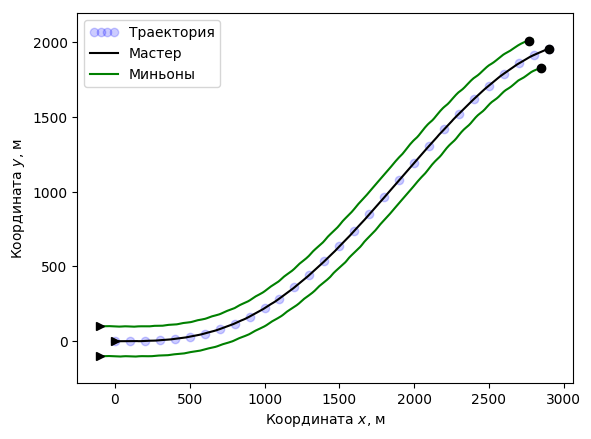
\includegraphics[width=0.7\linewidth]{platoon-trajectory-0}
	\caption{Движение строем мастера и двух миньонов}
	\label{fig:platoon-trajectory-0}
\end{figure}


\end{document}